\documentclass[a4paper,12pt]{report}
\usepackage{amsmath}
\usepackage{amssymb}
\usepackage{cancel}
%\usepackage{gensymb}
\usepackage{graphicx}
\usepackage{esint}
\usepackage{mdsymbol}
\usepackage{esvect} 
%\usepackage{lipsum}
\usepackage{hhline}
\usepackage{eurosym}
\usepackage{listings}
\usepackage{booktabs}
\usepackage{amssymb}
\usepackage{mathrsfs}
\usepackage{commath}
\usepackage{adjustbox}
\usepackage{booktabs}
\usepackage{array}
\usepackage{lscape}
\usepackage[xspace]{ellipsis}
\usepackage{color}
\usepackage{float}
\usepackage{caption}
\usepackage{afterpage}

\definecolor{mygreen}{rgb}{0,0.6,0}
\definecolor{mygray}{rgb}{0.5,0.5,0.5}
\definecolor{mymauve}{rgb}{0.58,0,0.82}
\begin{document}

\title{Master's Project Journal}
\author{Conor Dooley}
\maketitle
\section*{Initial Research}
The first week after I received my project was spent researching the concepts involved, mostly through the reading of papers and theses sent to me by my supervisors. These allowed me to gain an understanding as to why my project was needed, the technology that was involved and the goal of the project.
% I should probably make a thing in here regarding what these papers entailed?
% Non trivial however, reviewing those might be a better goal for a less busy period

%\subsection*{Paper 1}
\section*{D/NCO Research}
After my second supervisor meeting a goal was set for the following week of researching the potential designs for the Digitally/Numerically Controller Oscillator for this network. Going into this I was aware of two potential designs, one of these being a chain of inverters, which provided there was an odd number would oscillate with a period given by:
$$ 2\times\text{delay}\times n $$
Where $\text{delay}$ is the time taken for a signal pro propagate through an inverter and $n$ is the number of inverters in the chain.\\
The second option that I was aware of in advance of the research was a phase accumulator using a counter which would overflow at $2^n-1$ where $n$ is the bit width of the counter. By controlling the number that is added on each clock cycle of the main FPGA clock driving the counter the period of this oscillator can be adjusted.\\
The only other option I managed to come across for an oscillator on an FPGA was using Xilinx proprietary \texttt{IODELAY} blocks, which have a permanently programmable delay at runtime \ref{IODELAY}. This could be coupled with an odd number of inverters in order to implement a quasi ring oscillator. However as these are IO blocks their usage is not particularly conducive to the creation of a network of ADPLLs.
%\ref{IODELAY} https://www.xilinx.com/support/documentation/application_notes/xapp872.pdf
%After 2nd meeting with supervisors the goal was to find out what options there were in terms of implementing an oscillator on an FPGA. Only two real options were phase accumulator \& ring oscillator.

%Both of these I knew of in advance of this research. Xilinx proprietary option with IODelays. Goal for next week to implement an oscillator of both main options. %TODO Link papers & this section
\section*{Initial DCO Implementation}
Having analysed the potential options for the oscillator in this network we decided to implement both of the two viable options so my task for the week was to do this. The phase accumulator was easy to implement, just requiring a counter with an adjustable addition value.\\
The ring oscillator was more complicated although not because of the code itself being especially difficult, just requiring the use of a generate block to avoid having to type out the same line hundreds of times for each of the inverters required. The tricky part of this however was forcing Vivado to implement my verilog as written, as it wished to optimise away my inverter chains as it saw them as being redundant. The fact I had a combinatorial loop in my design presented it's own challenges in overcoming Vivado's complaints, especially as the net/cell names kept changing.\\
One of these problems came down to the usage of the incorrect Verilog keyword in order to prevent the optimisation of my inverters. I had taken this segment of the code from Brian's DSD notes and around the web many others had used the same directive in their code, \texttt{( * KEEP = true * )}, so some google-fu was required here.
Eventually I discovered that \texttt{KEEP} was limited to the synthesis and implementation stages hence my design working in timing simulations yet failing to be pass the generation of a bitstream.\\
I figured out that the correct directive was in fact \texttt{( * DONT\_TOUCH = true * )}, which while performing correctly and was able to carry on with fixing the combinatorial loop issue.\\
It turns out there is a \textit{simple} solution to the combinatorial loops problem as Vivado informs the user while reading the logs. However the suggested remedy of \newline
\texttt{set\_property ALLOW\_COMBINATORIAL\_LOOPS true [get\_nets \\<module\_hierarchy/net\_name>]}\newline
is not actually a functioning solution to this issue.
As it transpires the correct method is to select one of the cells that Vivado reports as being part of this loop and use this to locate the appropriate cell, shown in the following command.\newline
\texttt{set\_property ALLOW\_COMBINATORIAL\_LOOPS true [get\_nets -of\_objects [get\_cells <module\_hierarchy/cell\_name>]]}\newline
The other drawback of this method is that due to Vivado renaming cells and/or nets when the structure of the design changes the constraints are not automatically reapplied, however there may be a more generic way to implement this.

%Wrote Verilog in order to implement both a wave/inverter chain oscillator \& a counter based oscillator. Then made the test benches for these, only used post-synth simulation. Then implemented and tested. Counter based worked fine, runs perfectly @ generates divided clock. Wave seems to "toggle" an LED, but frequency is so high I cannot tell. Need to use a massive number of inverters, takes ages to synth \& therefore simulate. <- this seems to be vivado doing silly things. Turns out vivado is optimising away even with comb. loops allowed. Needed to faff around the .xdc file.

%Eventually went for 1000 -> gives 1.58 MHz w/ inv chain. Works as expected. ~315 ps gate delay.
\section*{Jitter detection}
Started the week attempting to implement a system using the FPGA to measure clock jitter. Prior to this I implemented the ability to tune the frequencies of the oscillators using the switches on the board. The ring oscillator was given 4 bit control, removing an extra pair of inverters each time, and an enable. As the phase accumulator has a naturally wide tuning range of to up half the clock frequency and the accumulator itself being 10 bits wide it made sense to give it 9 bit wide control as well as an enable.\\

I then attempted to implement the jitter detection on the FPGA itself. I ran into some issues with the crossing of clock domains and went to speak to Brian about it. While talking to him we came to the conclusion that the resolution offered by a detector on the FPGA would not offer a resolution high enough to accurately measure the jitter. For example at a 500 MHz FPGA clock, which is at the higher end of what is attainable, the period is 2 nano seconds. As things stand the delay through one inverter is approximately 315 picoseconds each one adds 0.63 nanoseconds to the period of the signal. At 5 MHz then:
$$ T_{nom} = 200\times10^{-9}\text{ ns ,}T_{next} = 202\times10^{-9}\text{ ns} $$
$$ F_{nom} = 5\times10^{6}\text{ Hz ,}F_{next} = 4.950495\times10^{-9}\text{ Hz} $$
$$ \Delta F_{FPGA} = 49.504\text{ kHz} $$
While the ring oscillators adjustment resolution is 1.26 nanoseconds given each step removes an inverter pair this is a change of 
$$ T_{nom} = 200\times10^{-9}\text{ ns ,}T_{next} = 201.26\times10^{-9}\text{ ns} $$
$$ F_{nom} = 5\times10^{6}\text{ Hz ,}F_{next} = 4.968697\times10^{-9}\text{ Hz} $$
$$ \Delta F_{RO} = 31.302\text{ kHz} $$
As the supposed jitter detector cannot even detect a change in the period by a step it is not a useful method for the detection of jitter.\\
In response to this we decided to do the jitter measurements used a 4 GS/s oscilloscope which has a resolution of 250 picoseconds, and following the same procedure this gives:
%...
$$ \Delta F_{Scope} = 6.24\text{ kHz} $$
which is a significant improvement and allows for a number of measurement points for each oscillator resolution step.\\

I then took a sample measurement of the clock output of the ring oscillator running at 5 MHz and began to process it in Matlab to get an idea of the jitter. To do this I wrote a basic script which calculated the mean and standard deviation of the periods in the sample as well and the Time Interval Error.
This week I also met with Eugene and demonstrated my code for him as well as giving him binary files containing 8 MSamp of data for both the ring oscillator and the phase accumulator. He will be able to analyse their jitter characteristics and from there begin to determine the optimum control coefficients.\\
Worked also with Pierre getting his oscillator to work, using a similar design to mine however implemented in VHDL.\\

\section*{OScope Control}
Over the weekend I attempted to establish whether the oscilloscope could be controlled from my computer to automate the data collection process, and having initially hit a dead end with the Agilent provided Matlab functionality I found some an implementation in \texttt{C} from a Professor in Nottingham.\\
I worked on this on Wednesday and hit roadblocks with direct wiring. I got from Brian a router and was, after some initial setup issues, to get basic communication going with the scope.
However when I attempted to extract the data from the oscilloscope I hit problems, a call to \texttt{new char[LEN]} was throwing a \texttt{std::Alloc} error which prevented the data actually being read back from the scope. 
I suspect this may possibly be due to the buffer I was attempting to create being 8 million elements or more in length. 
I intend trying this again tomorrow with reduced sizes and hopefully this will work. There is also the potential that rather than extracting the data I could use the scope's inbuilt save to USB in order to circumvent this problem.


\section*{MMCM Block}
After running into issues with the use of the reference 100 MHz clock via the on chip clock manager at the same time as using it for the Phase Accumulator I had made. Accordingly I resetup the MMCM block in order to generate both the buffered high frequency clock for the Phase Accumulator and the lower frequency 5 MHz signal \"required\" for the 7 segment display. Testing again proved that both could be run simultaneously, the benefit of in phase clocks being that crossing of clock domains does not need to be considered.

\section*{Phase Detection I}
The next step then was to work on a phase detection mechanism for the ADPLL. First off I went down the simplest route and implemented a 1 bit bang-bang detector using just a single D flip flop. After meeting with Brian on Wednesday we discussed some of the challenges of implementing the phase detector on an FPGA. Foremost among these was the issue of metastability and the likelihood of both signals occurring at the same time. For an implementation on an ASIC where an arbitration circuit can be constructed using gates I do not have this luxury, as I am restricted to simple look-up table elements. As a temporary workaround for this we decided I would implement a phase detector with the assumption that the signals are synchronised to the FPGA clock.\\
Working under this assumption I created a phase detector which counts the number of FPGA clock cycles between edges of the two signals in question. In order to avoid issues where the rising edge of the second signal detected occurs very shortly before the next rising edge of the first signal detected the maximum phase difference that can be detected is the high time of the first signal.\\
This phase detector outputs signed 2s complement integers that can be fed directly into the loop filter which succeeds this block.

The problem that this introduces then is the minimum phase difference detectable is 2.5 nano seconds which equates to a 65 KHz frequency or a 4.5$^\circ$ phase deviation.

\section*{Phase Detection II}
The above phase detector was created using a state machine with the following diagram describing its behaviour:\\
%TODO insert image of the state transitions
It is preceded by two synchronisers which attempt to avoid metastable conditions, which will be used for the time being so that I could advance until we found a method that worked more generally.\\
I was able to test this phase detector and confirm that it was measuring a frequency difference in line with what I expected given my simulation results, despite spending too much time trying to figure out why the display was not giving me a reasonable output when it was just being updated far too quickly to be human readable.\\
\begin{figure}[h]
    \centering
    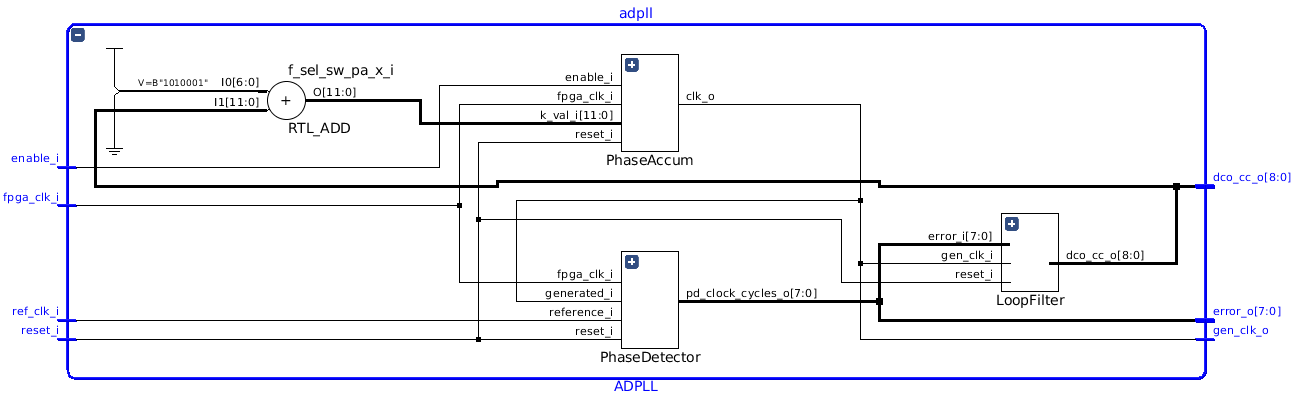
\includegraphics[scale=0.33]{../ADPLL_RTL_VIVADO}
    \caption{RTL Diagram of the ADPLL}
    \label{fig:adpll_rtl}
\end{figure}
I then realised I was also operating at a 160 MHz clock in both simulation and hardware so I attempted to push the clock up to the 400 MHz mark then but started to run into so timing issues on both inter and intra clock paths so I had to dial back the FPGA clock frequency to 258 MHz which was enough to remove all but what I think is an allowable timing violation on a synchroniser.\\
Working with the 1:0.1 rule for proportional/integral gains I then implemented a PI loop filter as in Eldar's PhD on Friday in order to complete an entire multi-bit ADPLL.
After ironing out one issue caused by a lack of bit extension causing strange behaviour on the control code if it was negative which had gone undetected in simulation I was able to get my PLL locking to an on-chip reference signal late on Friday.
In more detail the 8 bit signed output of the error loop filter was being added to a 12 bit bias signal and due to a lack of sign extension -1 became a +511. This error would correct itself on the next cycle leading to signal which looked like: $||--|||||-----||--|||||$\\r
Pierre told me about his method for the arbiter so maybe I can implement that method myself rather than relying on my limited use case version.

\begin{figure}[h]
    \centering
    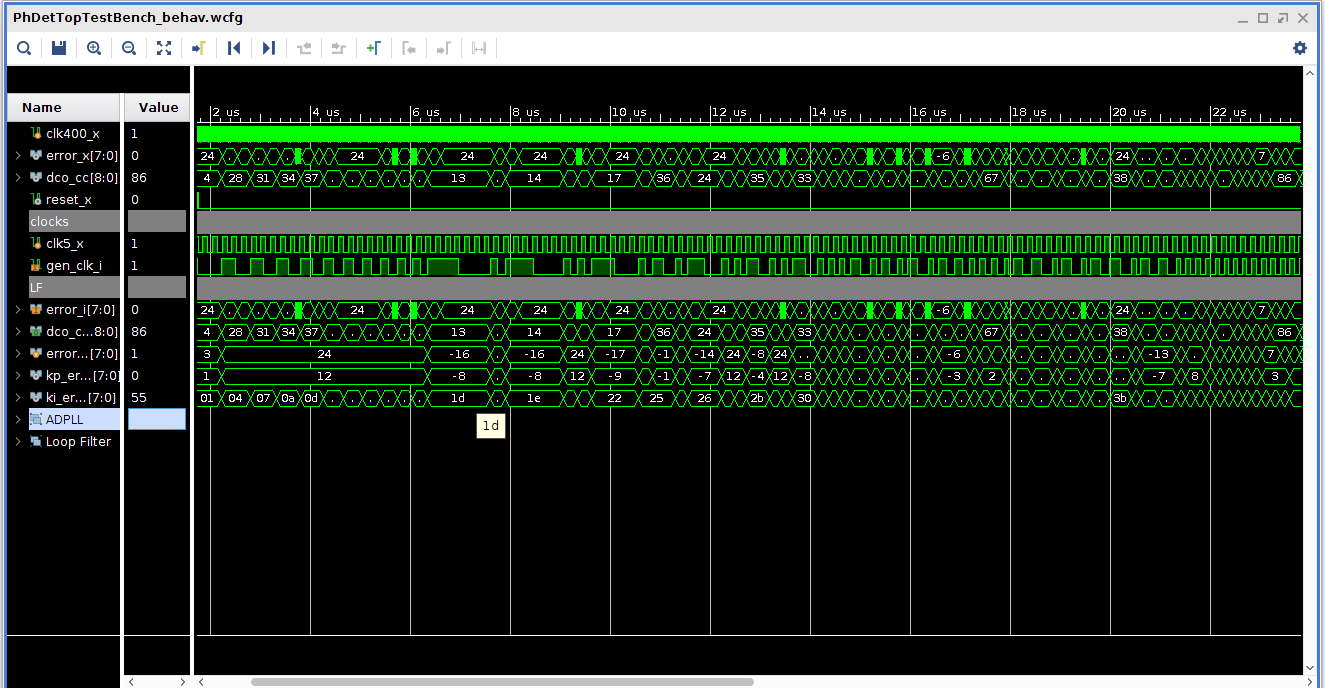
\includegraphics[scale=0.33]{../good_sim}
    \caption{Example simulation}
    \label{fig:example_sim}
\end{figure}

\section*{Basic Measurements}
Lock range at bias of 82:
$$4.19\rightarrow12.34\textrm{ MHz} $$ 
Capture range at bias of 82:
$$4.25\rightarrow12.76\textrm{ MHz}  $$
Jitter at bias of 82:\\
$$ 200.1665\pm1.9689\textrm{ nsec} $$
Jitter locked to 5~ MHz:\\
$$ 200.009\pm2.7378\textrm{ nsec} $$
Frequency sensitivity(control code to output):
$$ 258\times10^6\frac{1}{2^{12}}=62.988\textrm{ MHz} $$
Overall proportional gain (time $\rightarrow$ TDC $\rightarrow$ frequency):
$$ 8.998 \textrm{ KHz/degree} $$
LPF cutoff:\\

\begin{figure}[h]
    \centering
    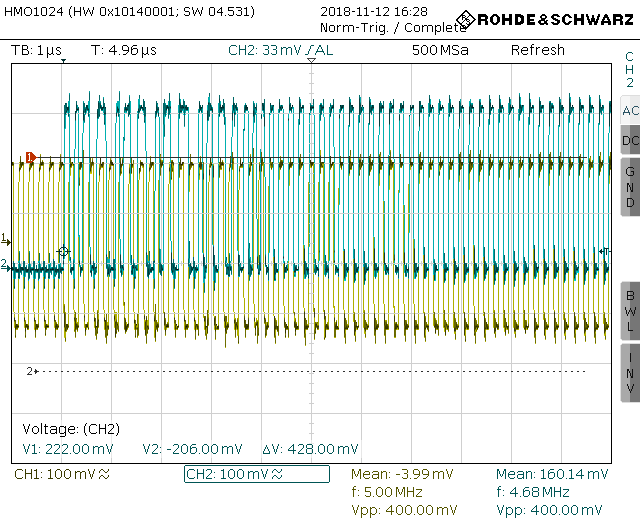
\includegraphics[scale=0.33]{../HMO_locking_4M7_to5M0}
    \caption{Example of locking at startup}
    \label{fig:hmo_locking}
\end{figure}%redo on good scope

\section*{RingADPLL}
Had to change the number of inverters significantly as it the new layout since my last test of a significantly more simple system had a different layout, especially only 8 steps of 2 inverters rather than 32 in this design which \texttt{OscTestTopLevel} used with a raw Bang Bang Phase Detector. Unfortunately all simulations broke and I was not actually able to simulate this re calibration of the ``bias''(really the number of inverters) and had to do it manually by generating bit streams and seeing how high low I could pull the frequency of operation.

\section*{External Reference}
I was able to simply re purpose an Arduino PWM script I had previously made as the reference. I then was able to run the ADPLL at 10 MHz from a reference at 1.25 MHz. The choice to run at 10 rather than 5 Meg was due to instability that was introduce with a division by eight to use the reference and a resulting inability to actually lock without reducing the clock frequency of the phase detection circuit (4x required for 8x reference scaling). I also made some large changes to the Loop Filter to allow for gain variation both in width and value.

\section*{Truncation in 2s Complement (LF)}
This is an issue that needs addressing. I am truncating and that may corrupt the number. For now it doesn't matter however it may with certain configurations.

\section*{RingOsc Sim Issue}
For some reason I cannot run simulations of anything other than the RingOsc module itself. Any high level module fails to simulate properly, seemingly zero delay oscillation once the chain is enabled.

\section*{External Reference II}
Problem was with the offset of the reference, once fixed things worked as expected. I previously had it zero centred rather than zero-min

\section*{Gain Testing}
Varied gains to find lower jitter operation. Required fixing of the loop filter truncation. Optimal gain changed significantly based on the configuration in use.

\section*{Chained PLLs}
Chained together 2 PLLs and the reference as so:
\begin{equation*}
	ref -> pll1 <=> pll2
\end{equation*}
required the creation of a weighted error combiner. Moved the PFD out of the PLL block for reuse between neighbours.

\section*{Baby's First Floorplanning}
Did things with floorplanning in order to ensure the ring oscillator doesnt change its frequency all the time.

\section*{Ring Osc}
Tried to get this into a PLL and lock to the reference. Struggled for ~6 hours with it and never got close to locking.

\section*{2x2 Network}
Tried this w/ PA PLL,  couldnt get locking, got something that was "close" to locked with huge amounts of jitter. Will attempt to locate the issue tomorrow. Potentially there is an error in the PLL, or a missing error negation.
	



\end{document}
